\section{Increasing Abstraction}

A new model has emerged that departs from the standard approach of
emulating an expanded HFS over increasingly greater geographies. This
model allows applications to treat data as an abstraction: opaque
objects that present little to no detail about the underlying data.
Rather than a hierarchy of directories and files, this model presents
the illusion of a flat object store. Applications submit data of
arbitrary type and are returned a unique ``handle'' to the data that
allows later data retrieval without requiring any greater understanding
of the underlying mechanisms used to store, protect, validate, and
retrieve the data; essentially creating a ``write once, read
everywhere'' method of operation. Details of where or how a given object
is stored are self-contained within the object store itself. Therefore,
the object store inherits all responsibility for data location,
integrity, and immutability. The application is successfully divorced
from the business of file location and management.

\subsection{A Brief History of Abstraction in the Data
Center}

Computer science has steadily sought to increase abstraction as a
principal means of advancement. In the IT space this is evidenced by the
move from a monolithic system that performed all functions to an
increasing dispersion of function across multiple devices. Individual
devices are thus allowed to be less complex while gaining increasing
sophistication in the smaller set of tasks for which the device is
purpose built.

Initially, all computing resources were stored and performed in a single
monolithic structure. All service depended upon access to the central
site. A failure with the central computing element resulted in a
complete black-out of all service. Further, the complexity of the
central computing element was necessarily quite complex as it had to
have native intelligence to perform every function
(Figure~\ref{fig:monolithic}).

\begin{figure}[htbp]
\centering
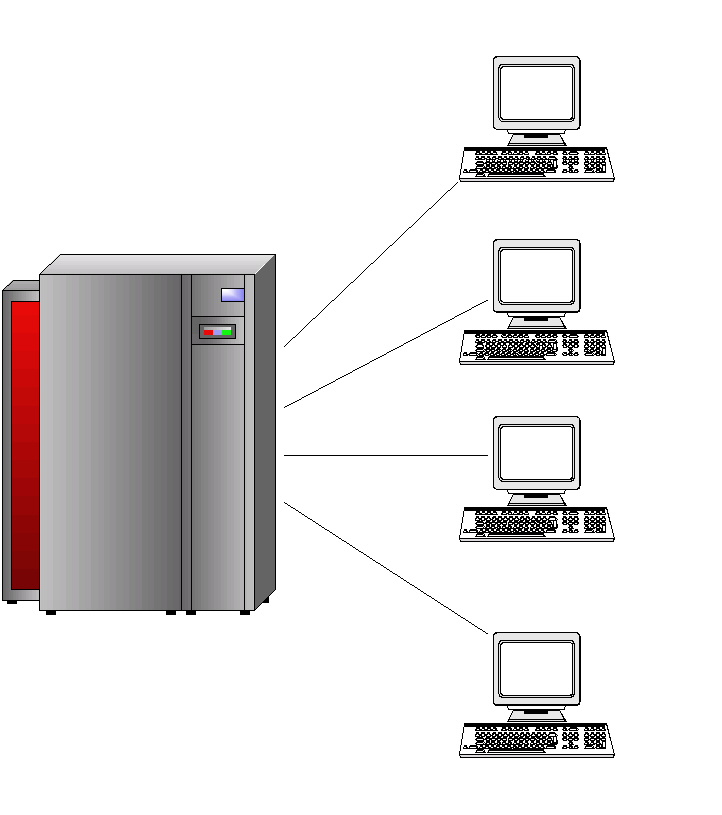
\includegraphics[width=0.58\linewidth,height=0.45373\linewidth]{fig/monolithic.jpg}
\caption{Monolithic Structure}\label{fig:monolithic}
\end{figure}


Over time it became evident that there were efficiencies to be gained
from separating the \emph{presentation} of data from its
\emph{execution}. This lead to a 2-tiered model commonly referred to as
client-server, where the client had principal responsibility for the
``presentation layer'' and the server held principal responsibility for
the ``execution layer.'' While this model provided some efficiencies,
both in application programming and in purpose-built appliances, there
remained a tight coupling between the execution server and the data
store, as depicted in Figure~\ref{fig:client-server}.

\begin{figure}[htbp]
\centering
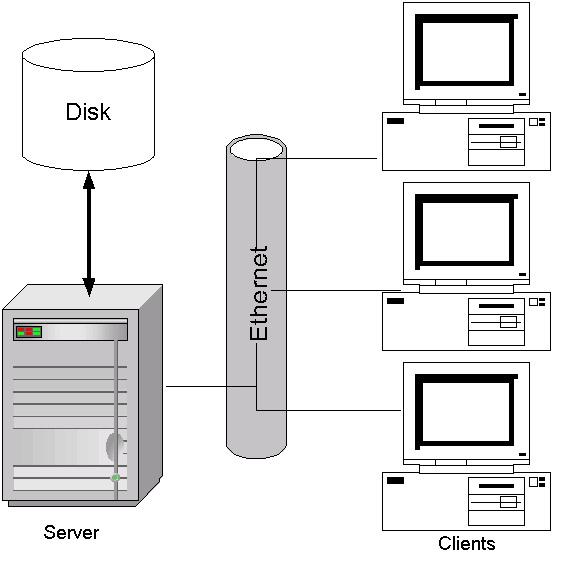
\includegraphics[width=0.58\linewidth]{fig/client-server.jpg}
\caption{Client / Server Architecture}\label{fig:client-server}
\end{figure}


The next logical stepwise function was to separate the data store from
the execution layer. This led to the advancement of the 3-tier (also
referred to as the \emph{N}-tiered) model, as depicted in
Figure~\ref{fig:client-server-server}.

\begin{figure}[htbp]
\centering
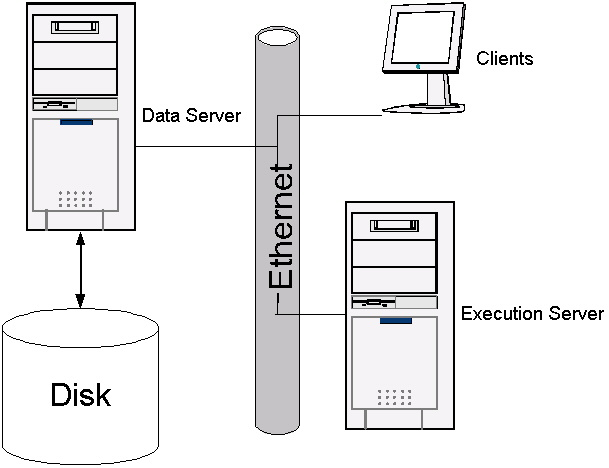
\includegraphics[width=0.58\linewidth]{fig/client-server-server.jpg}
\caption{Client / Server / Server Architecture}\label{fig:client-server-server}
\end{figure}


While architecturally sound in principal, the \emph{N}-tiered model
never achieved its full potential in practice as applications operating
at the execution layer are not truly separated from the details of the
data store. While physically separate, there remains an incestuous
relationship between the applications that execute upon the data and the
details of how data is stored.

This failure to meet the ideal of the \emph{N}-tiered abstraction model
is not simply an academic distinction. To the extent that the
application developer, and by extension IT operations, must be concerned
about the detail of data, they are distracted from performing the task
at hand. For further progress to be made the ideal of \emph{N}-tiered
model must be realized. The alternative is relative stagnation, with
only marginal gains in application development.

\subsection{Completing the Ideal}

The model of universal object store represents a quantum step forward in
the goal to increase abstraction to the point where application
developers are all but completely relieved of the details of data
storage. While this significantly reduces the burden on the application
developer, it has the beneficial side-effect of reducing IT complexity.
The exposed and often fragile link between applications and the file(s)
they use is broken, thus allowing IT greater flexibility in the
organization - and more importantly re-organization - of data. IT Ops
benefits as well as this additional layer of abstraction eliminates the
block/file distinction for managing data, which causes so many headaches
for IT managers and end users \cite{ref3}. Further, by introducing
sophisticated software within the object store that owns all aspects of
data storage and its management, this effectively moves ``storage'' up
the value chain, both to the application developer and IT Operations.

\subsection{Protection from Changes in Physical
Mediums}

This degree of abstraction provides protection not only in the important
area of abstracting file location, but in the area of physical medium as
well. It is a given that physical mediums will continue to change over
time. HDD's continue to live on, despite predictions of their demise,
and continue to improve density at impressive rates. Nonetheless, it's
certain that this curve cannot extend indefinitely; eventually further
meaningful density improvements will become impossible. Given the
physics of the medium it is estimated that areal density of HDD's will
reach maximum possible density at
\textasciitilde150Gb/in\textsuperscript{2}. At which point the problem
of superparamagnetism\footnote{When maximum areal density is reached,
  the magnetic energy holding the bits in place on the medium becomes
  equal to the ambient thermal energy within the disk drive itself. When
  this happens, the bits are no longer held in a reliable state and can
  "flip," scrambling the data that was previously recorded.} is expected
to prohibit future HDD density increases.

Regardless of precisely \emph{when} it occurs, it is generally
acknowledged that it will become necessary to move to storage mediums
beyond the 2-dimensional, with work on 3-dimensional light (holograms)
as storage medium already begun. Whatever the medium, the opaque nature
of the object store protects applications from eventual changes in the
medium.

\subsection{The Payoff}

The benefits of abstraction in computer science and electrical
engineering have long been understood. Abstraction can reasonably be
attributed with providing the foundation necessary for future
achievement; both in computer hardware and software. Kernel-based HFS's
have provided application developers a sound data abstraction model for
more than three decades. However, with the addition of an increasing
numbers of file servers dispersed over increasing geographies, file
management complexity continues to increase geometrically.

Application developers and IT Operations alike need a refinement of this
classic model to effectively deal with massive quantities of data. The
advent of commercial-grade object store technology, coupled with
dramatic advancements in disk price/performance, makes it possible for
IT organizations to keep ahead of the complexity curve in a
cost-effective manner.
